\documentclass[11pt]{article}
\usepackage[textwidth=18.0cm, textheight=23.0cm, top=2.0cm]{geometry}
\usepackage{pst-all}
\usepackage{amssymb}
\usepackage{tikz}
\usepackage{underscore}\begin{document}
\pagestyle{empty}


ClassName: \underline{\textbf{Class_07.2bp-27}}
\par
BinSize: \underline{\textbf{100 × 100}}
\par
ReduceSize: \underline{\textbf{100 × 100}}
\par
TypeNum: \underline{\textbf{59}}
\par
Num: \underline{\textbf{60}}
\par
OutS: \underline{\textbf{170000}}
\par
InS: \underline{\textbf{145305}}
\par
Rate: \underline{\textbf{0.855}}
\par
UB: \underline{\textbf{17}}
\par
LB0: \underline{\textbf{17}}
\par
LB: \underline{\textbf{17}}
\par
LBWithCut: \underline{\textbf{17}}
\par
NodeCut: \underline{\textbf{0}}
\par
ExtendedNodeCnt: \underline{\textbf{1}}
\par
GenNodeCnt: \underline{\textbf{1}}
\par
PrimalNode: \underline{\textbf{0}}
\par
ColumnCount: \underline{\textbf{17}}
\par
TotalCutCount: \underline{\textbf{0}}
\par
RootCutCount: \underline{\textbf{0}}
\par
LPSolverCnt: \underline{\textbf{1}}
\par
PricingSolverCnt: \underline{\textbf{0}}
\par
BranchAndBoundNum: \underline{\textbf{1}}
\par
isOpt: \underline{\textbf{true}}
\par
TimeOnInitSolution: \underline{\textbf{0.770 s}}
\par
TimeOnPrimal: \underline{\textbf{0.000 s}}
\par
TimeOnPricing: \underline{\textbf{0.000 s}}
\par
TimeOnRmp: \underline{\textbf{0.062 s}}
\par
TotalTime: \underline{\textbf{0.895 s}}
\par
\newpage


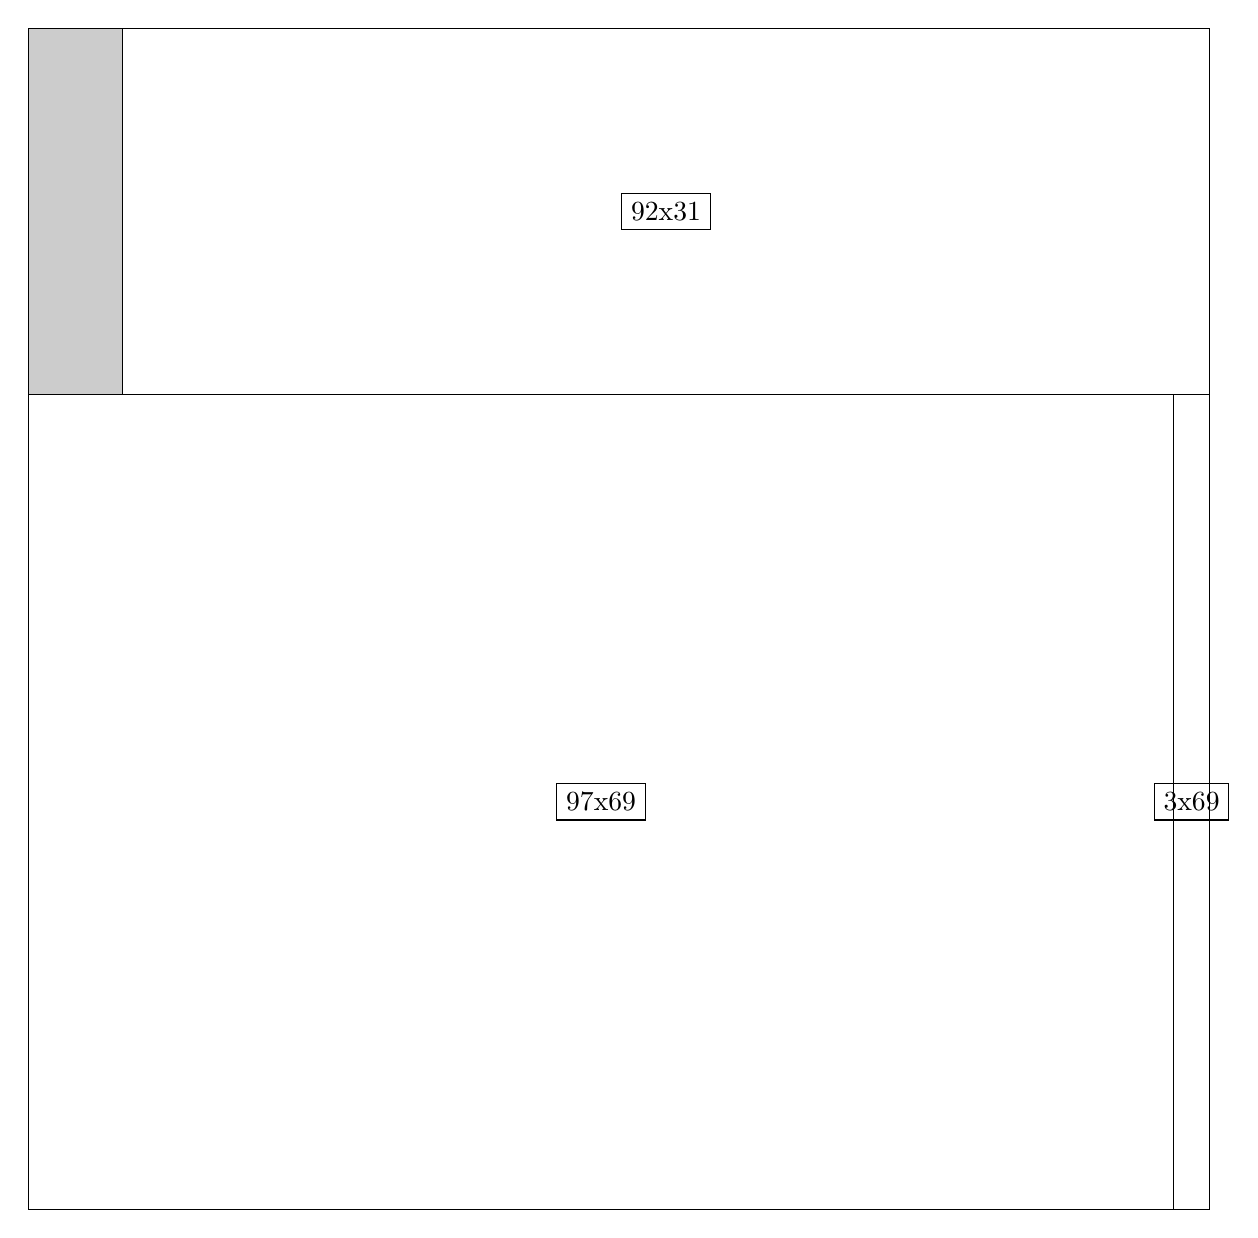
\begin{tikzpicture}[shorten >=1pt,scale=1.0,every node/.style={scale=1.0},->]
\tikzstyle{vertex}=[circle,fill=black!25,minimum size=14pt,inner sep=0pt]
\filldraw[fill=gray!40!white, draw=black] (0,0) rectangle (15.0,15.0);
\foreach \name/\x/\y/\w/\h in {97x69/0.0/0.0/14.549999999999999/10.35,92x31/1.2/10.35/13.799999999999999/4.6499999999999995,3x69/14.549999999999999/0.0/0.44999999999999996/10.35}
\filldraw[fill=white!40!white, draw=black] (\x,\y) rectangle node[draw] (\name) {\name} ++(\w,\h);
\end{tikzpicture}


w =97 , h =69 , x =0 , y =0 , v =6693
\par
w =92 , h =31 , x =8 , y =69 , v =2852
\par
w =3 , h =69 , x =97 , y =0 , v =207
\par
\newpage


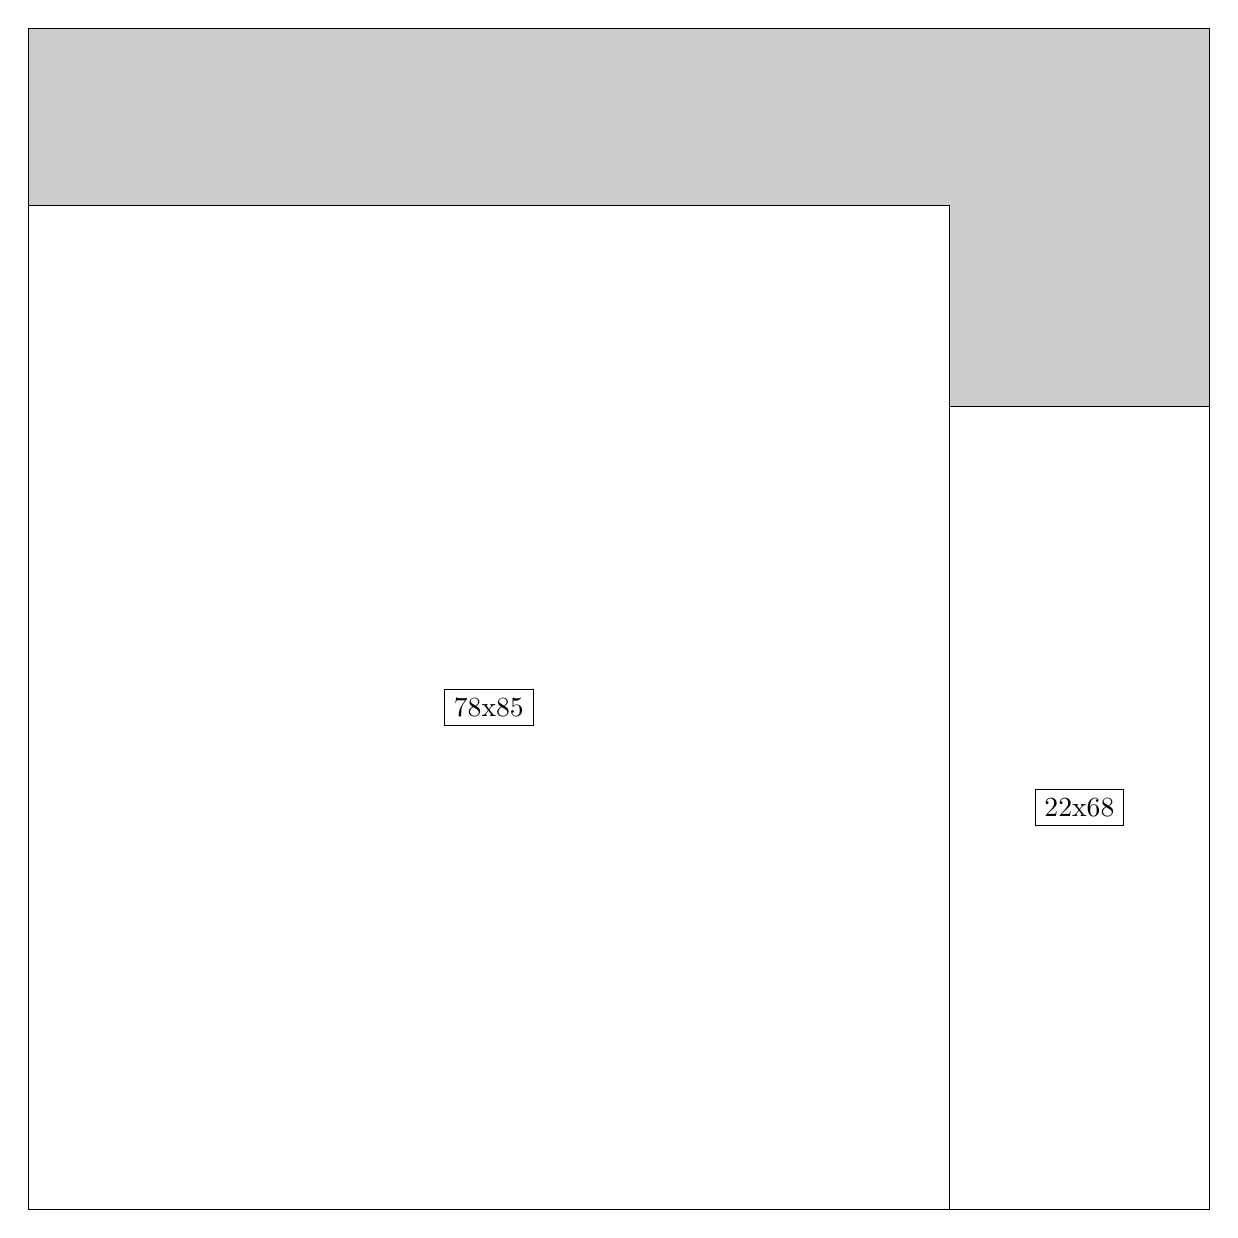
\begin{tikzpicture}[shorten >=1pt,scale=1.0,every node/.style={scale=1.0},->]
\tikzstyle{vertex}=[circle,fill=black!25,minimum size=14pt,inner sep=0pt]
\filldraw[fill=gray!40!white, draw=black] (0,0) rectangle (15.0,15.0);
\foreach \name/\x/\y/\w/\h in {22x68/11.7/0.0/3.3/10.2,78x85/0.0/0.0/11.7/12.75}
\filldraw[fill=white!40!white, draw=black] (\x,\y) rectangle node[draw] (\name) {\name} ++(\w,\h);
\end{tikzpicture}


w =22 , h =68 , x =78 , y =0 , v =1496
\par
w =78 , h =85 , x =0 , y =0 , v =6630
\par
\newpage


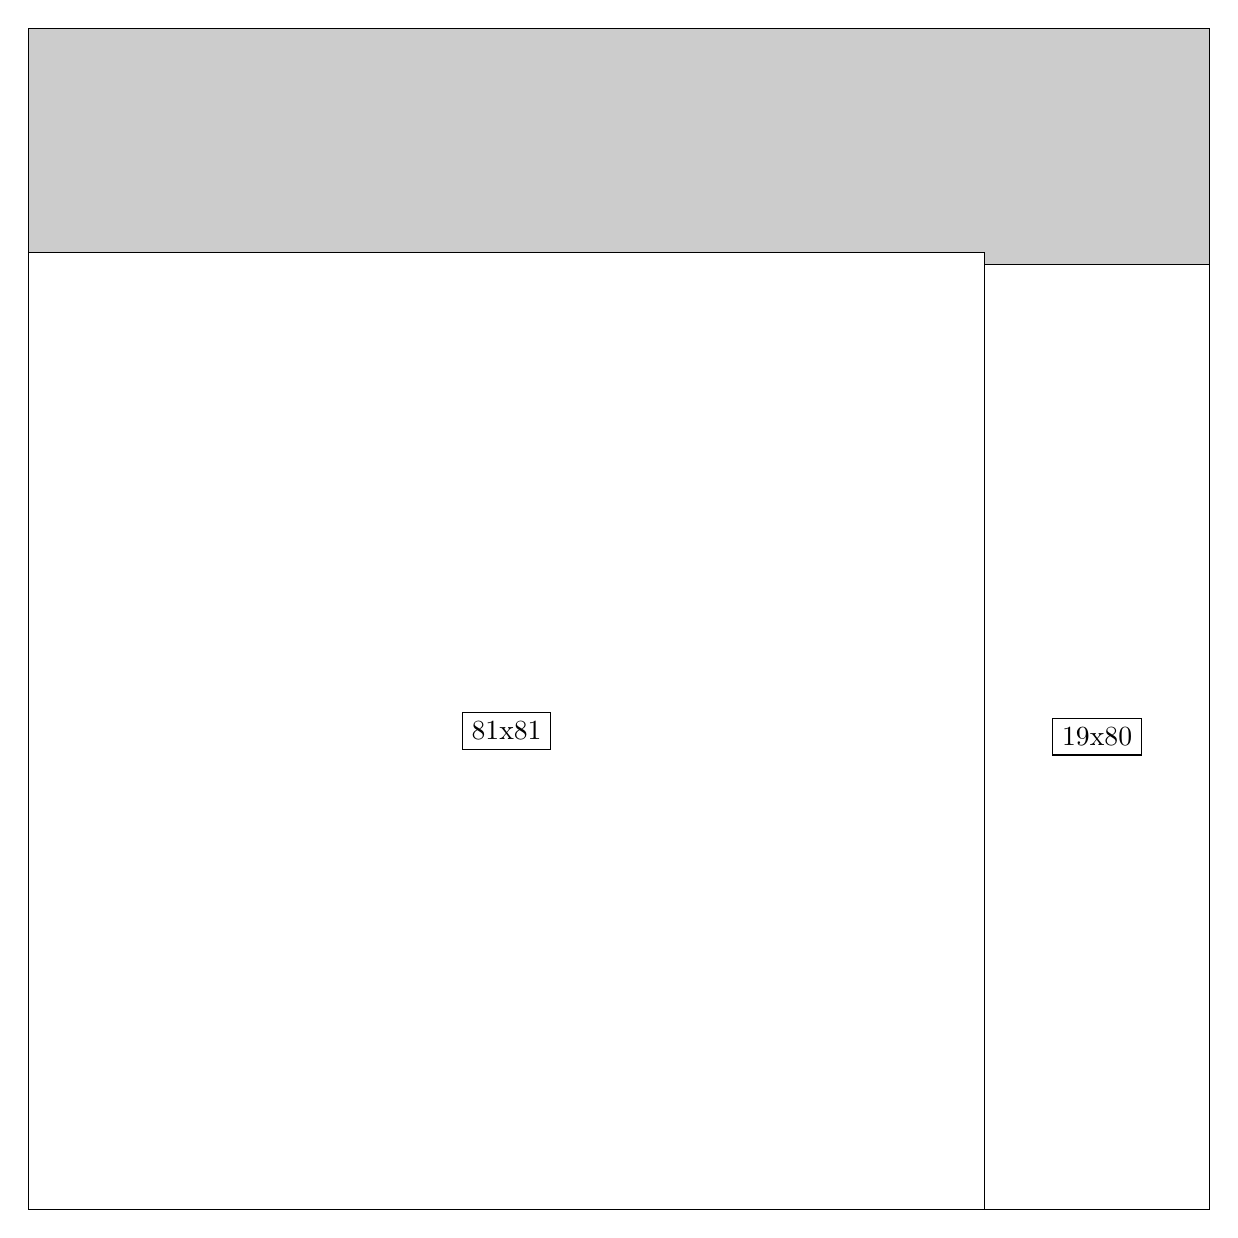
\begin{tikzpicture}[shorten >=1pt,scale=1.0,every node/.style={scale=1.0},->]
\tikzstyle{vertex}=[circle,fill=black!25,minimum size=14pt,inner sep=0pt]
\filldraw[fill=gray!40!white, draw=black] (0,0) rectangle (15.0,15.0);
\foreach \name/\x/\y/\w/\h in {81x81/0.0/0.0/12.15/12.15,19x80/12.15/0.0/2.85/12.0}
\filldraw[fill=white!40!white, draw=black] (\x,\y) rectangle node[draw] (\name) {\name} ++(\w,\h);
\end{tikzpicture}


w =81 , h =81 , x =0 , y =0 , v =6561
\par
w =19 , h =80 , x =81 , y =0 , v =1520
\par
\newpage


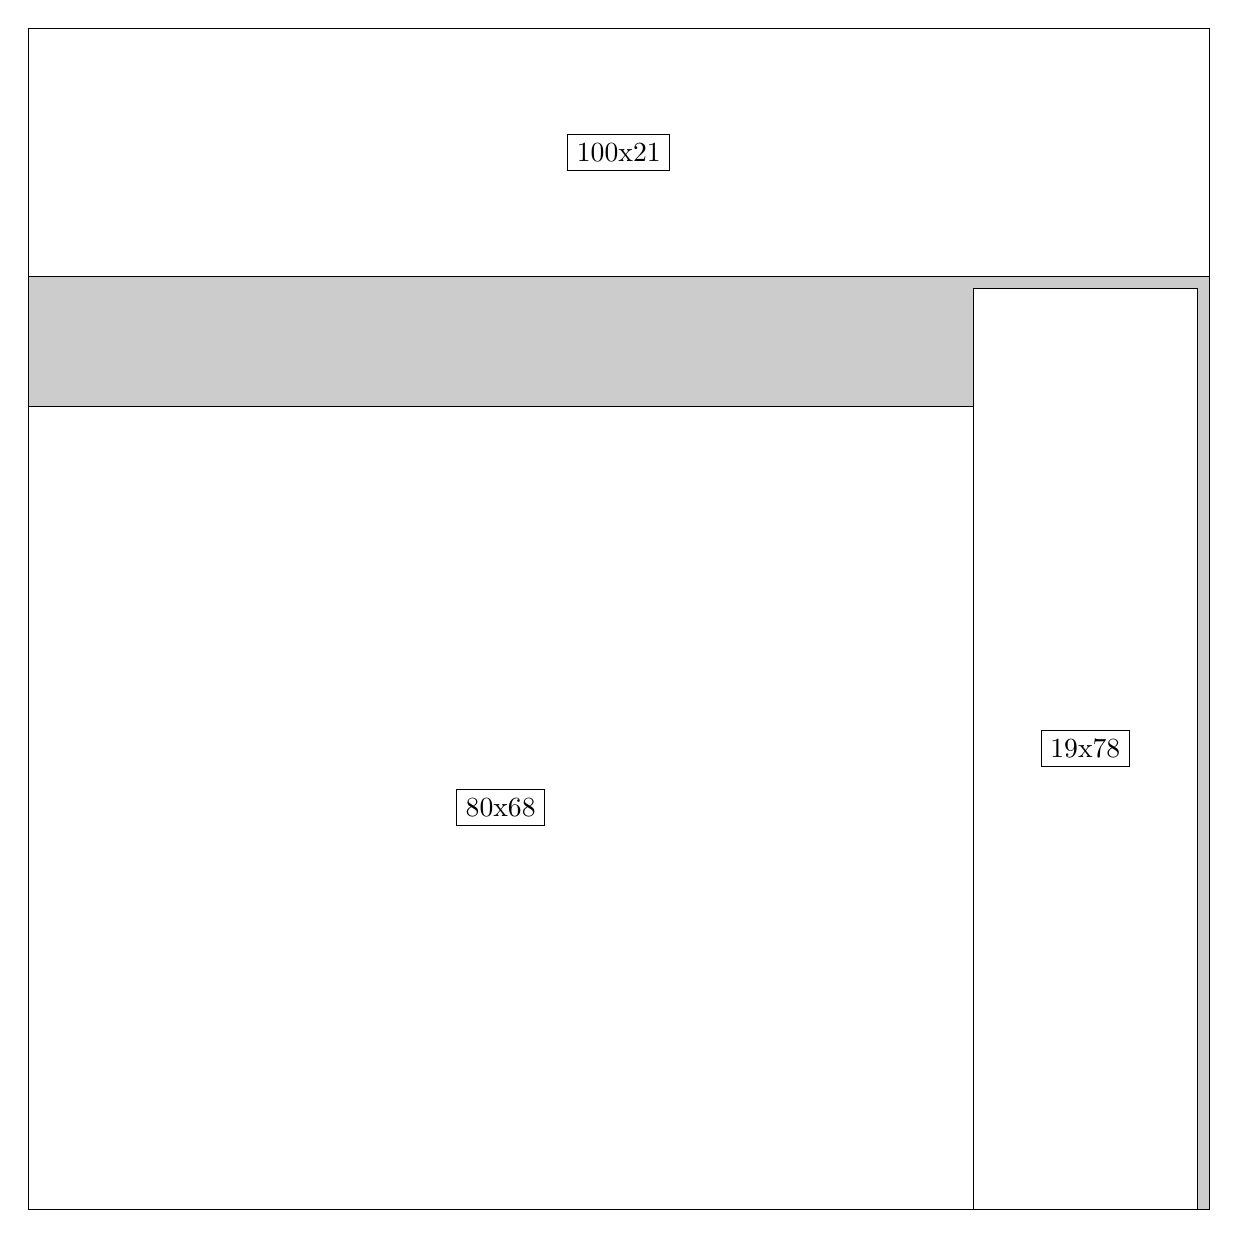
\begin{tikzpicture}[shorten >=1pt,scale=1.0,every node/.style={scale=1.0},->]
\tikzstyle{vertex}=[circle,fill=black!25,minimum size=14pt,inner sep=0pt]
\filldraw[fill=gray!40!white, draw=black] (0,0) rectangle (15.0,15.0);
\foreach \name/\x/\y/\w/\h in {80x68/0.0/0.0/12.0/10.2,19x78/12.0/0.0/2.85/11.7,100x21/0.0/11.85/15.0/3.15}
\filldraw[fill=white!40!white, draw=black] (\x,\y) rectangle node[draw] (\name) {\name} ++(\w,\h);
\end{tikzpicture}


w =80 , h =68 , x =0 , y =0 , v =5440
\par
w =19 , h =78 , x =80 , y =0 , v =1482
\par
w =100 , h =21 , x =0 , y =79 , v =2100
\par
\newpage


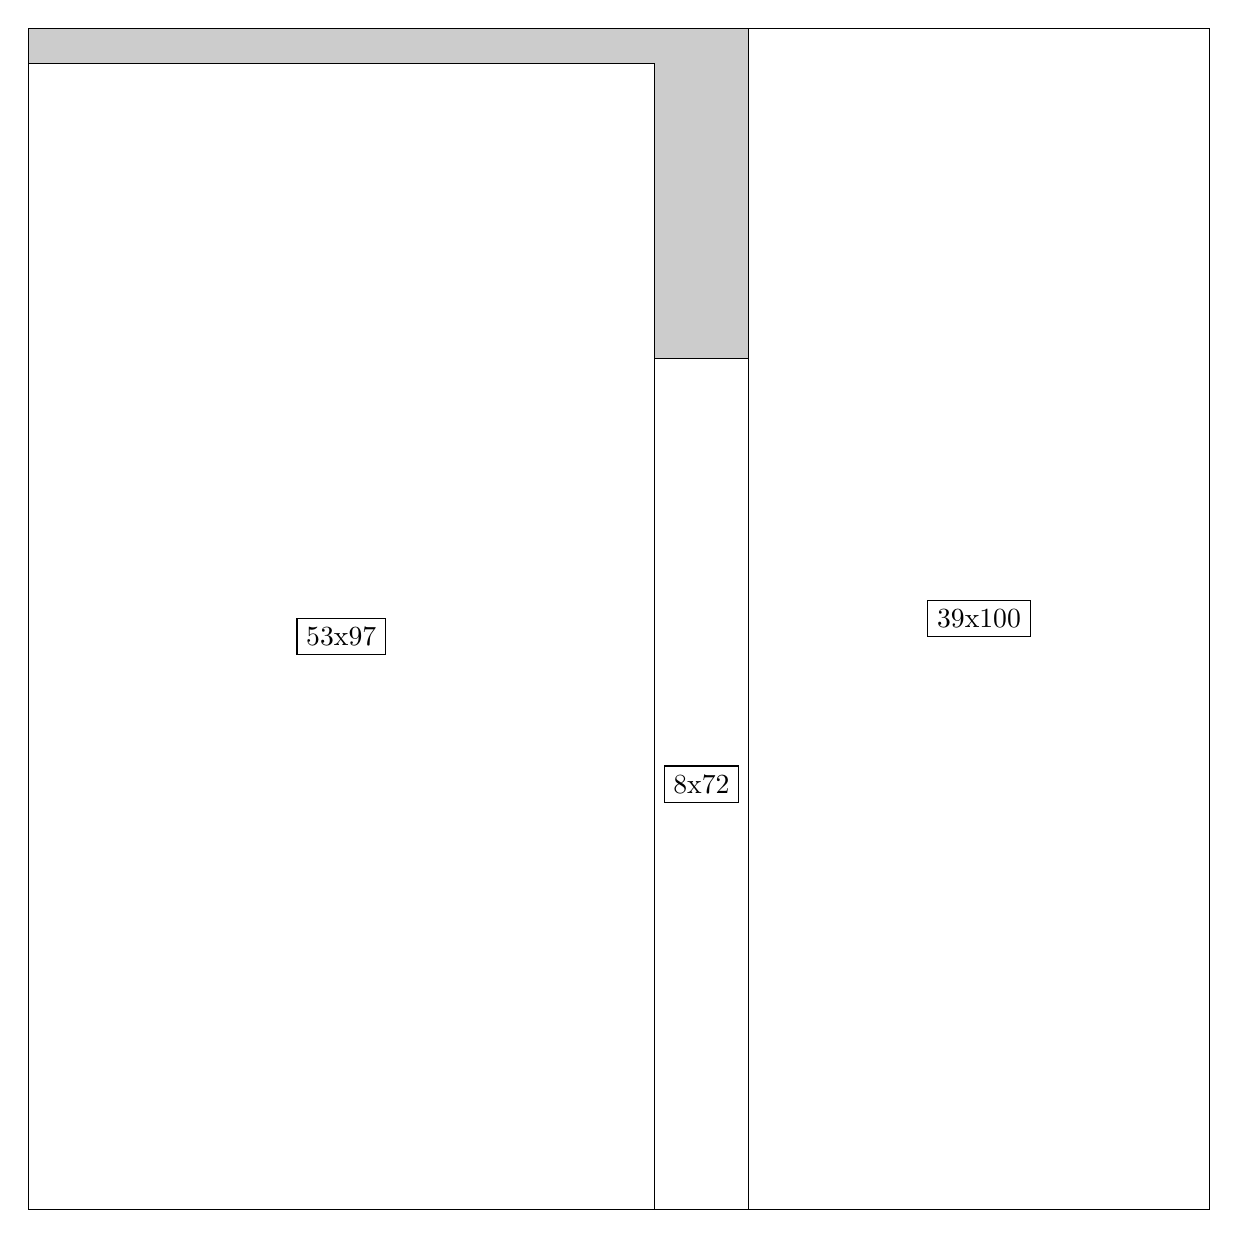
\begin{tikzpicture}[shorten >=1pt,scale=1.0,every node/.style={scale=1.0},->]
\tikzstyle{vertex}=[circle,fill=black!25,minimum size=14pt,inner sep=0pt]
\filldraw[fill=gray!40!white, draw=black] (0,0) rectangle (15.0,15.0);
\foreach \name/\x/\y/\w/\h in {53x97/0.0/0.0/7.949999999999999/14.549999999999999,39x100/9.15/0.0/5.85/15.0,8x72/7.949999999999999/0.0/1.2/10.799999999999999}
\filldraw[fill=white!40!white, draw=black] (\x,\y) rectangle node[draw] (\name) {\name} ++(\w,\h);
\end{tikzpicture}


w =53 , h =97 , x =0 , y =0 , v =5141
\par
w =39 , h =100 , x =61 , y =0 , v =3900
\par
w =8 , h =72 , x =53 , y =0 , v =576
\par
\newpage


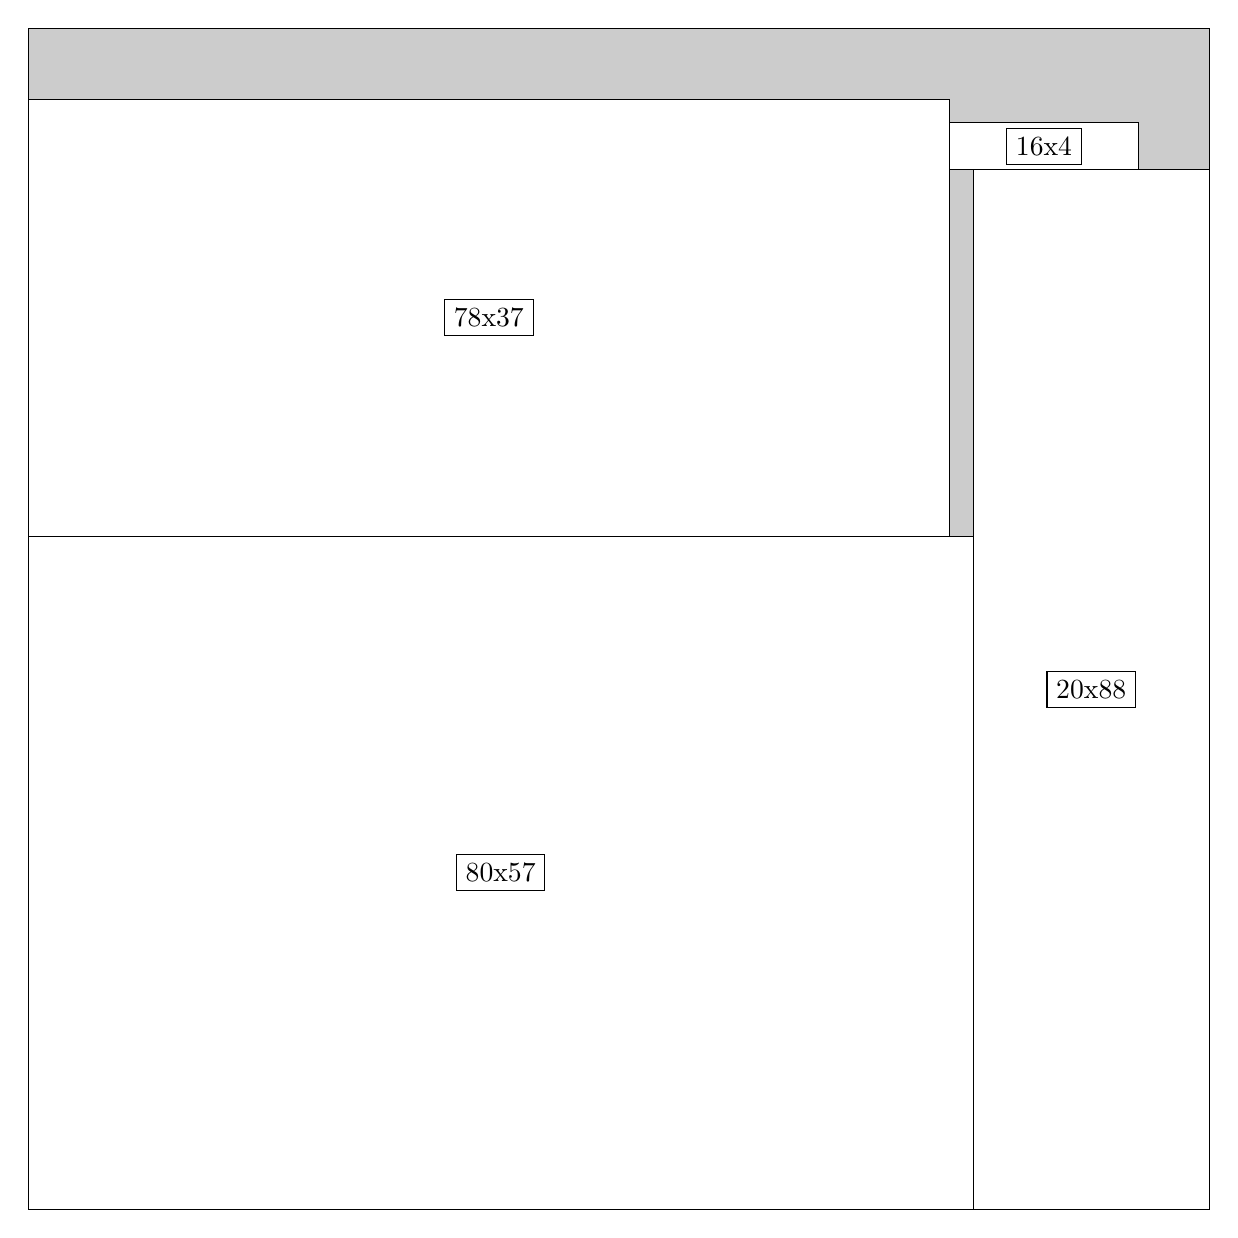
\begin{tikzpicture}[shorten >=1pt,scale=1.0,every node/.style={scale=1.0},->]
\tikzstyle{vertex}=[circle,fill=black!25,minimum size=14pt,inner sep=0pt]
\filldraw[fill=gray!40!white, draw=black] (0,0) rectangle (15.0,15.0);
\foreach \name/\x/\y/\w/\h in {80x57/0.0/0.0/12.0/8.549999999999999,78x37/0.0/8.549999999999999/11.7/5.55,20x88/12.0/0.0/3.0/13.2,16x4/11.7/13.2/2.4/0.6}
\filldraw[fill=white!40!white, draw=black] (\x,\y) rectangle node[draw] (\name) {\name} ++(\w,\h);
\end{tikzpicture}


w =80 , h =57 , x =0 , y =0 , v =4560
\par
w =78 , h =37 , x =0 , y =57 , v =2886
\par
w =20 , h =88 , x =80 , y =0 , v =1760
\par
w =16 , h =4 , x =78 , y =88 , v =64
\par
\newpage


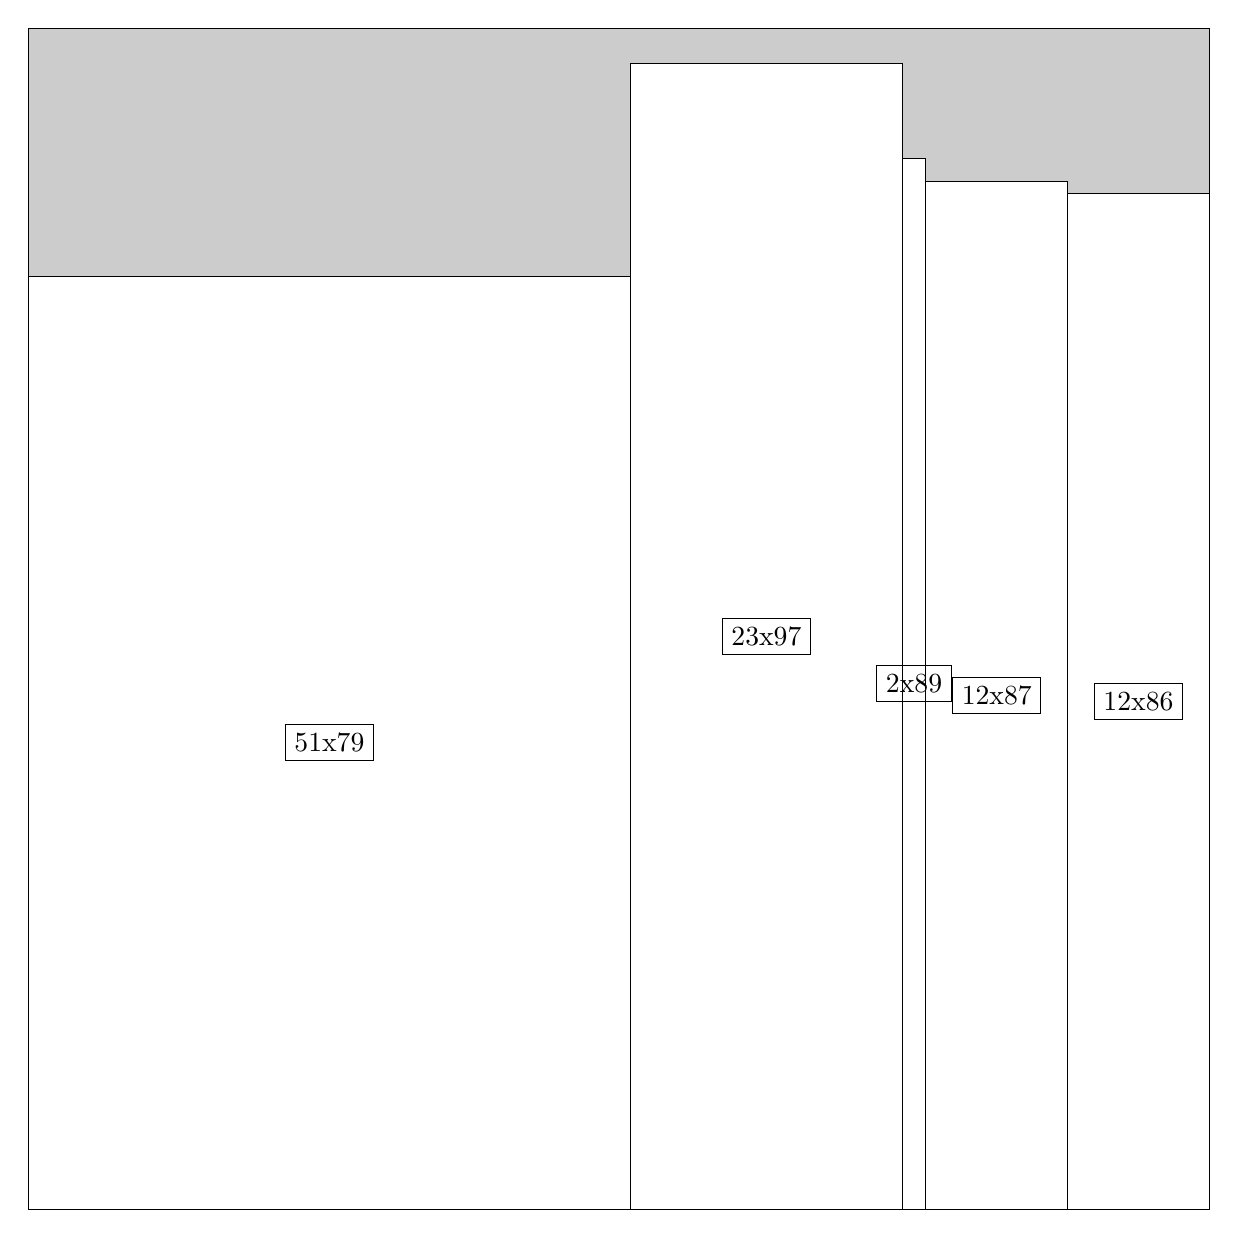
\begin{tikzpicture}[shorten >=1pt,scale=1.0,every node/.style={scale=1.0},->]
\tikzstyle{vertex}=[circle,fill=black!25,minimum size=14pt,inner sep=0pt]
\filldraw[fill=gray!40!white, draw=black] (0,0) rectangle (15.0,15.0);
\foreach \name/\x/\y/\w/\h in {51x79/0.0/0.0/7.6499999999999995/11.85,23x97/7.6499999999999995/0.0/3.4499999999999997/14.549999999999999,12x87/11.4/0.0/1.7999999999999998/13.049999999999999,12x86/13.2/0.0/1.7999999999999998/12.9,2x89/11.1/0.0/0.3/13.35}
\filldraw[fill=white!40!white, draw=black] (\x,\y) rectangle node[draw] (\name) {\name} ++(\w,\h);
\end{tikzpicture}


w =51 , h =79 , x =0 , y =0 , v =4029
\par
w =23 , h =97 , x =51 , y =0 , v =2231
\par
w =12 , h =87 , x =76 , y =0 , v =1044
\par
w =12 , h =86 , x =88 , y =0 , v =1032
\par
w =2 , h =89 , x =74 , y =0 , v =178
\par
\newpage


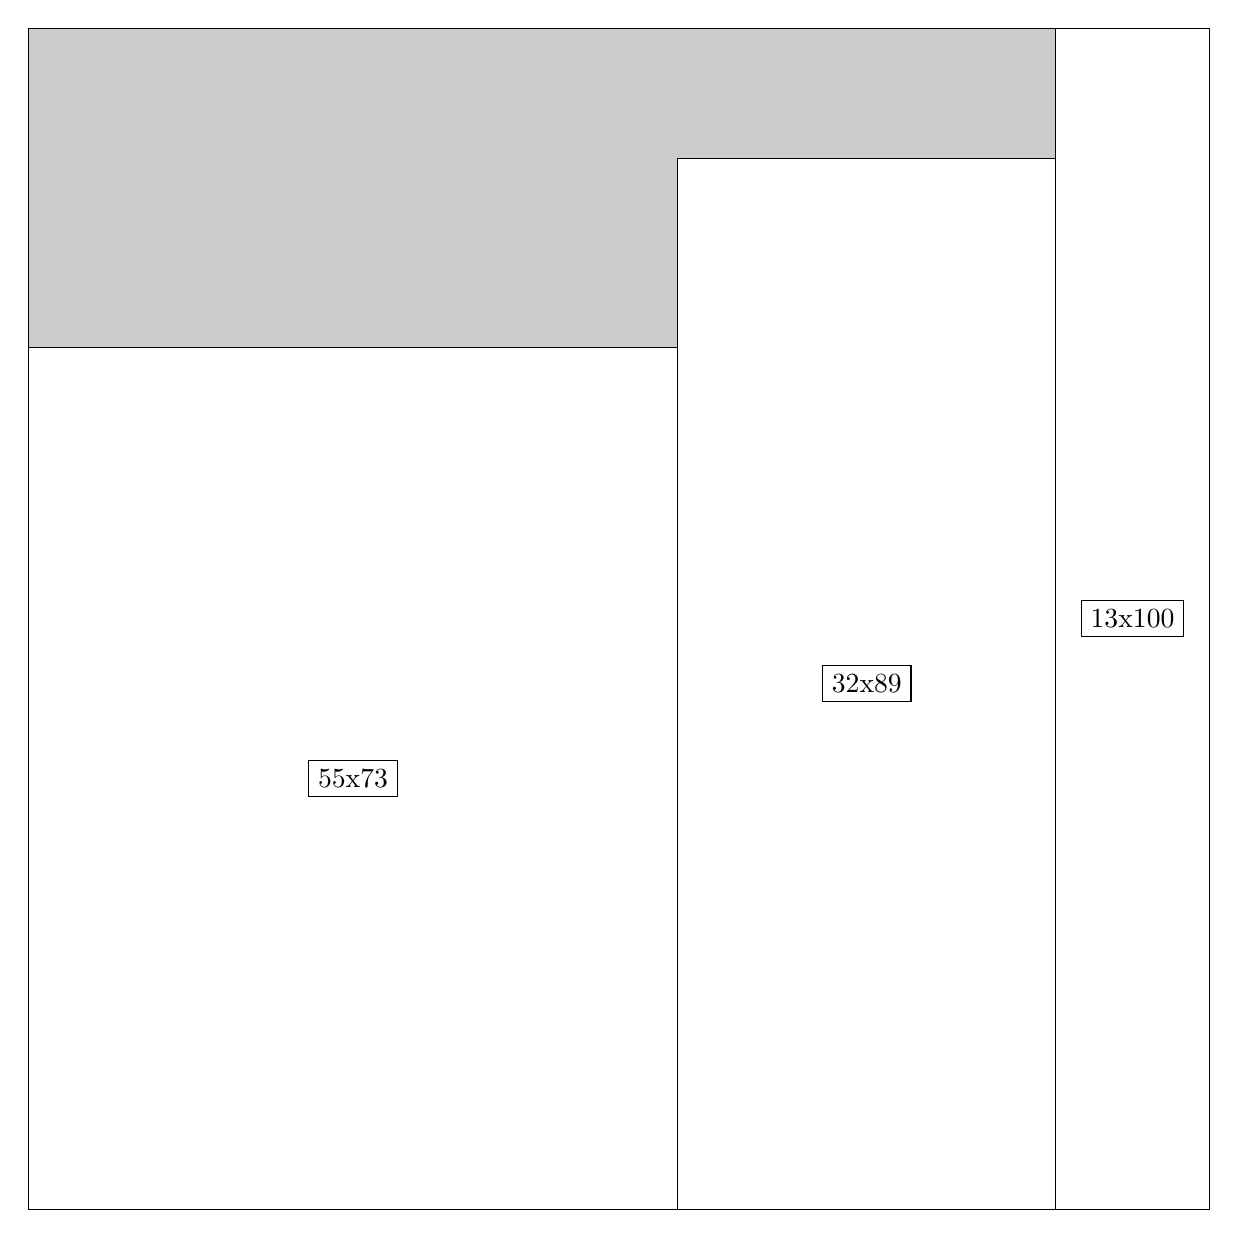
\begin{tikzpicture}[shorten >=1pt,scale=1.0,every node/.style={scale=1.0},->]
\tikzstyle{vertex}=[circle,fill=black!25,minimum size=14pt,inner sep=0pt]
\filldraw[fill=gray!40!white, draw=black] (0,0) rectangle (15.0,15.0);
\foreach \name/\x/\y/\w/\h in {55x73/0.0/0.0/8.25/10.95,32x89/8.25/0.0/4.8/13.35,13x100/13.049999999999999/0.0/1.95/15.0}
\filldraw[fill=white!40!white, draw=black] (\x,\y) rectangle node[draw] (\name) {\name} ++(\w,\h);
\end{tikzpicture}


w =55 , h =73 , x =0 , y =0 , v =4015
\par
w =32 , h =89 , x =55 , y =0 , v =2848
\par
w =13 , h =100 , x =87 , y =0 , v =1300
\par
\newpage


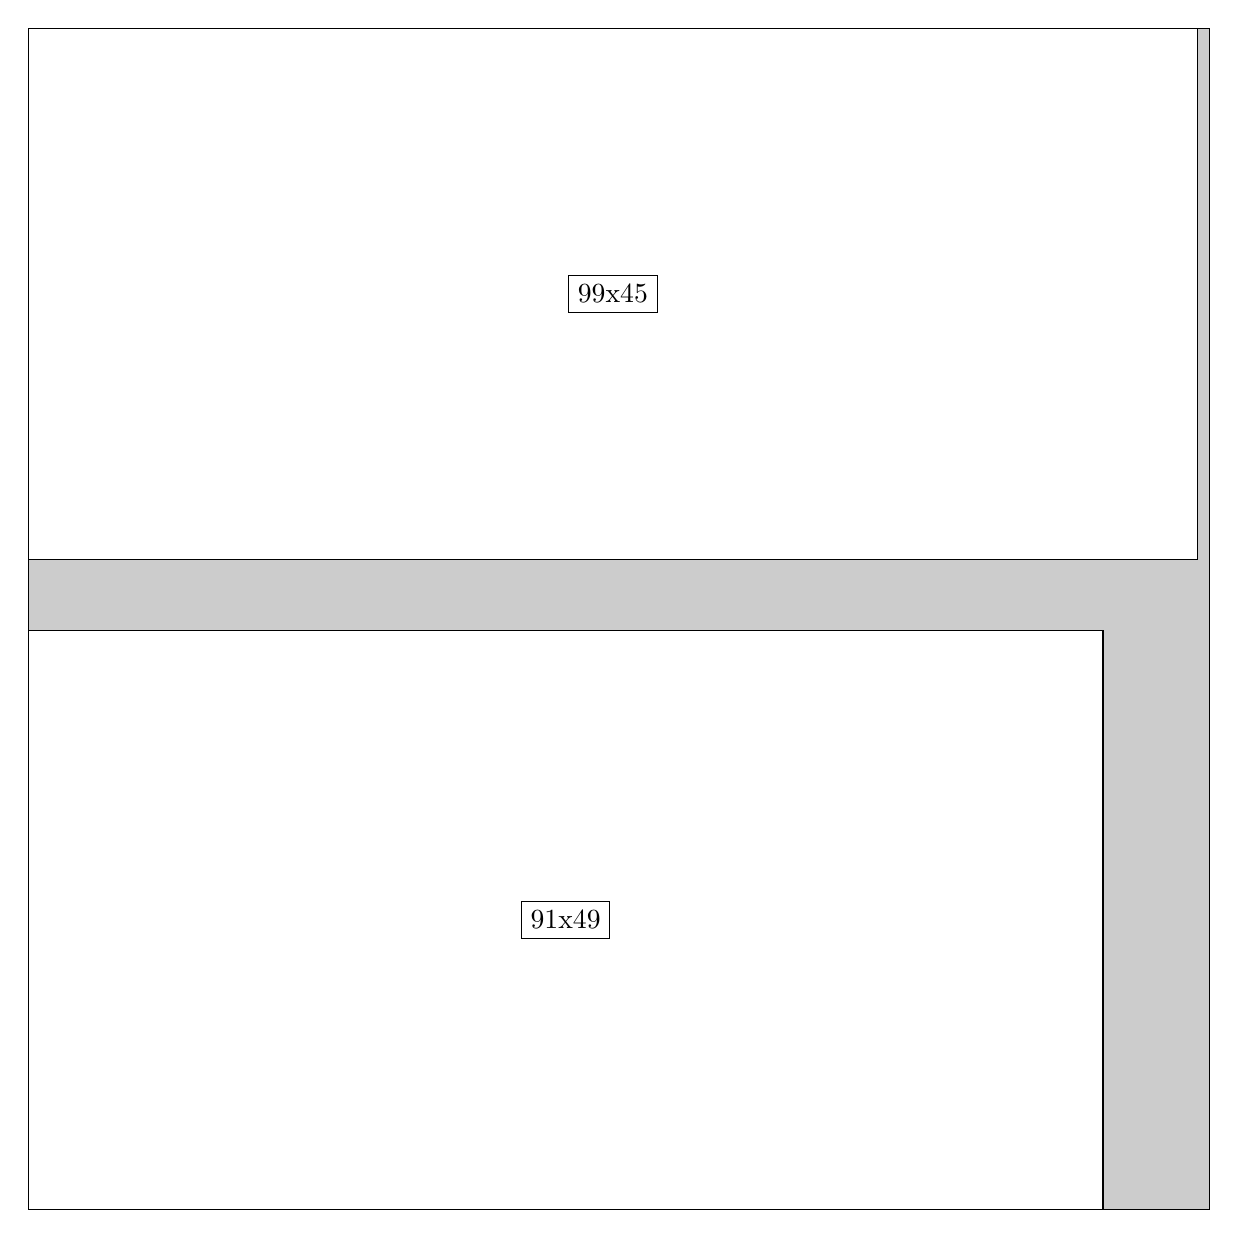
\begin{tikzpicture}[shorten >=1pt,scale=1.0,every node/.style={scale=1.0},->]
\tikzstyle{vertex}=[circle,fill=black!25,minimum size=14pt,inner sep=0pt]
\filldraw[fill=gray!40!white, draw=black] (0,0) rectangle (15.0,15.0);
\foreach \name/\x/\y/\w/\h in {91x49/0.0/0.0/13.65/7.35,99x45/0.0/8.25/14.85/6.75}
\filldraw[fill=white!40!white, draw=black] (\x,\y) rectangle node[draw] (\name) {\name} ++(\w,\h);
\end{tikzpicture}


w =91 , h =49 , x =0 , y =0 , v =4459
\par
w =99 , h =45 , x =0 , y =55 , v =4455
\par
\newpage


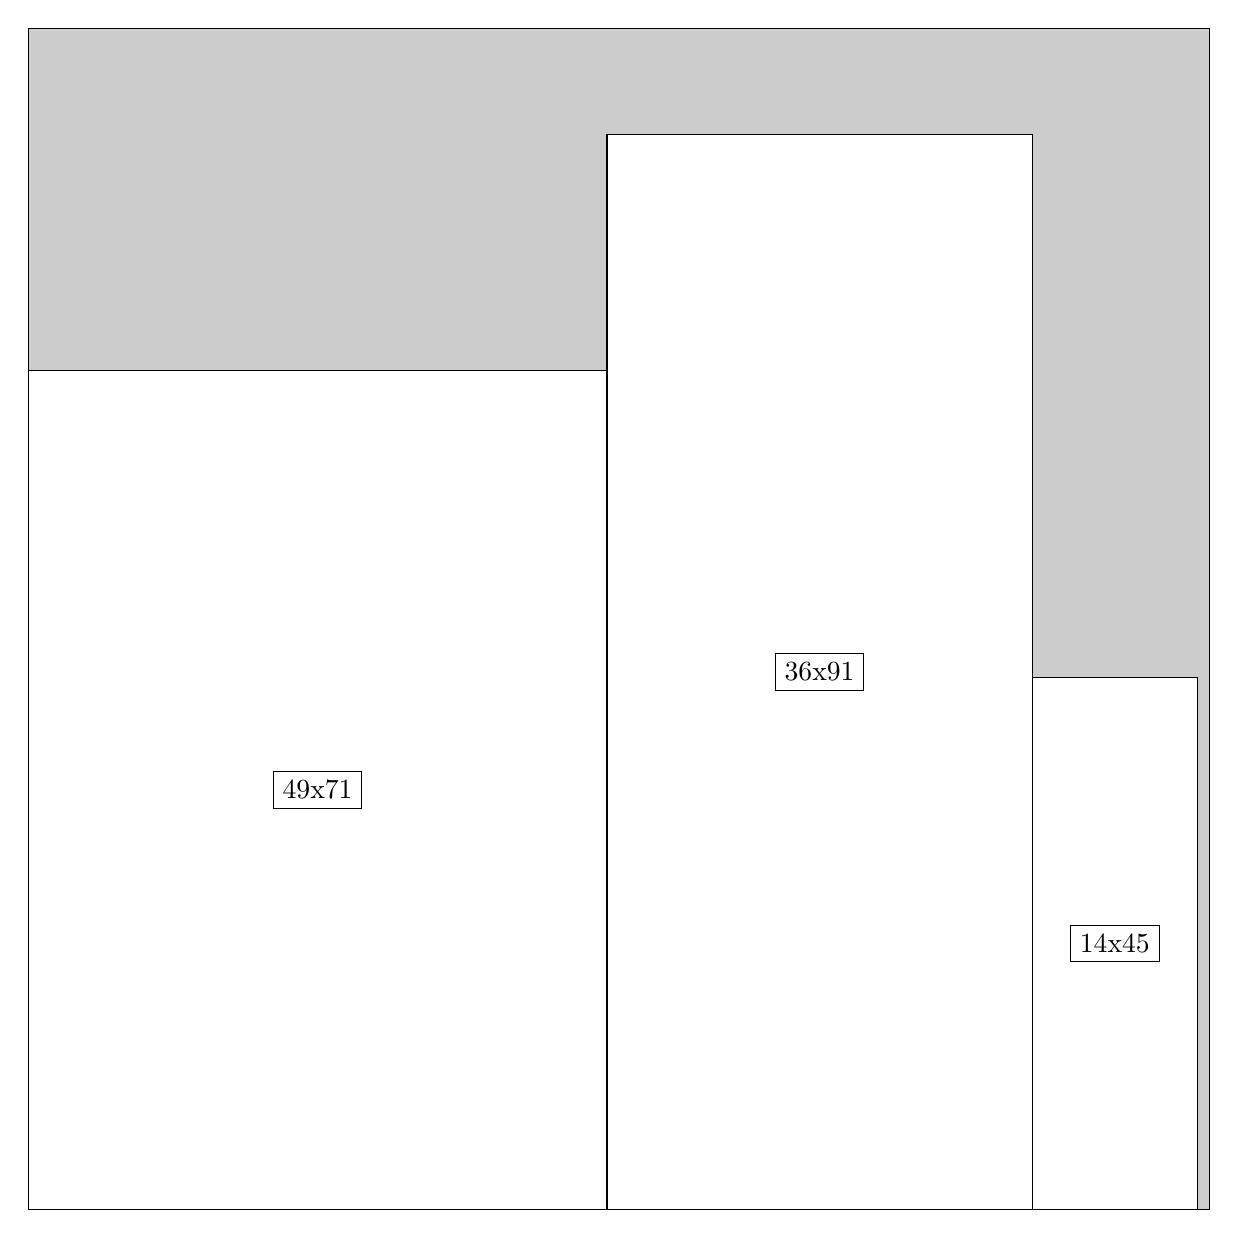
\begin{tikzpicture}[shorten >=1pt,scale=1.0,every node/.style={scale=1.0},->]
\tikzstyle{vertex}=[circle,fill=black!25,minimum size=14pt,inner sep=0pt]
\filldraw[fill=gray!40!white, draw=black] (0,0) rectangle (15.0,15.0);
\foreach \name/\x/\y/\w/\h in {49x71/0.0/0.0/7.35/10.65,36x91/7.35/0.0/5.3999999999999995/13.65,14x45/12.75/0.0/2.1/6.75}
\filldraw[fill=white!40!white, draw=black] (\x,\y) rectangle node[draw] (\name) {\name} ++(\w,\h);
\end{tikzpicture}


w =49 , h =71 , x =0 , y =0 , v =3479
\par
w =36 , h =91 , x =49 , y =0 , v =3276
\par
w =14 , h =45 , x =85 , y =0 , v =630
\par
\newpage


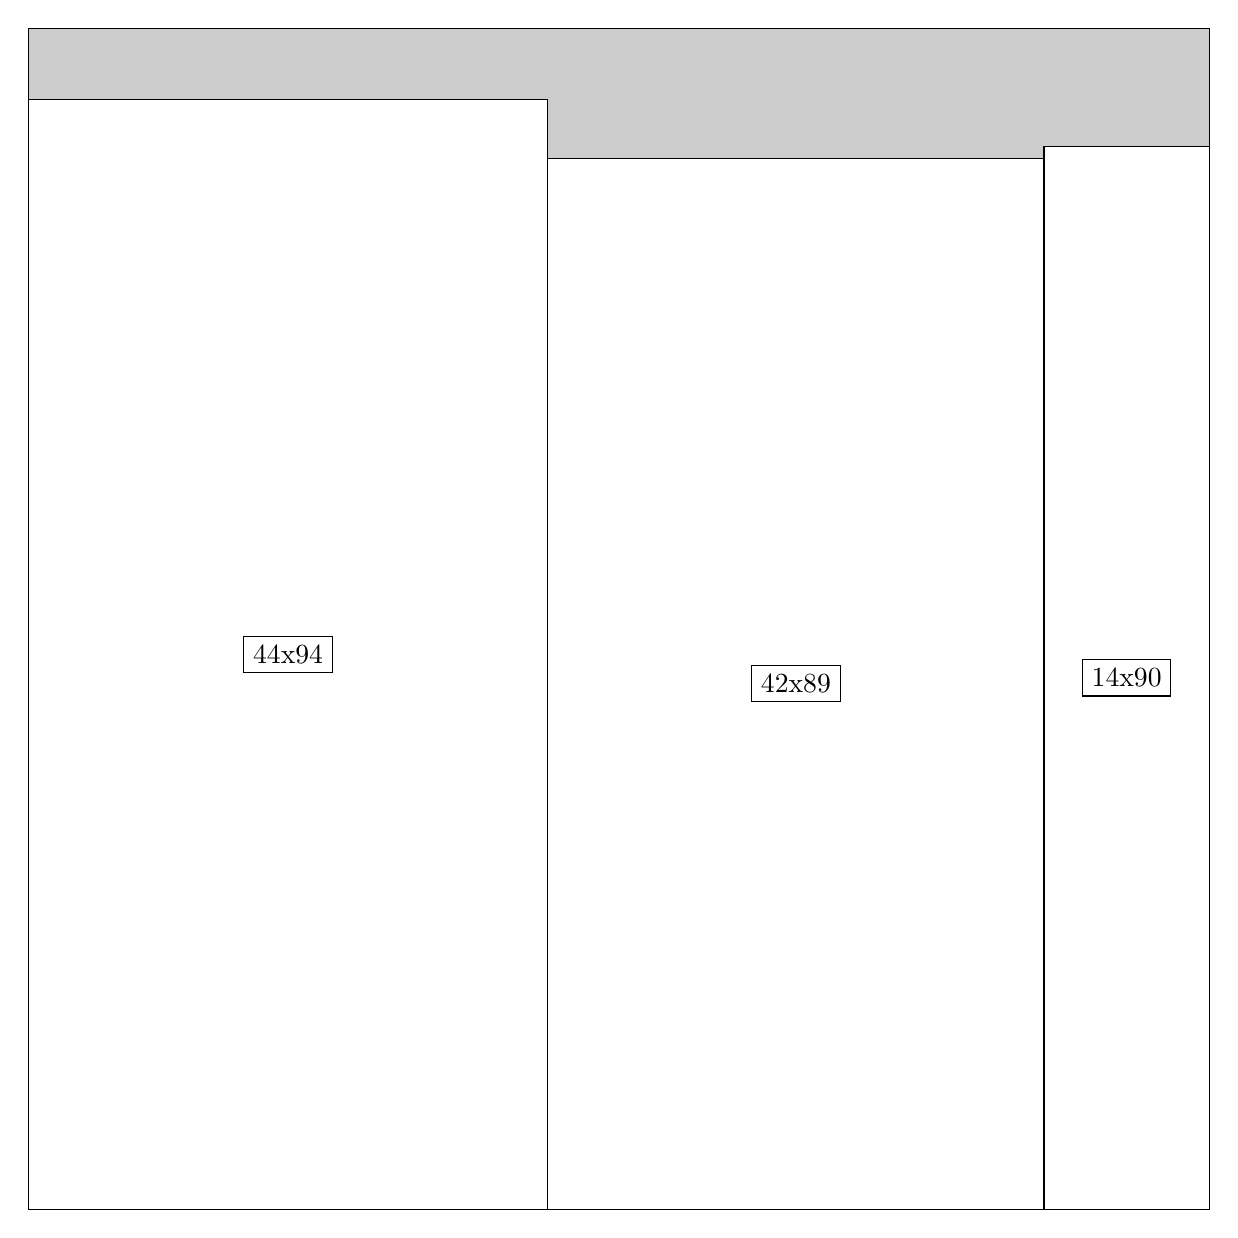
\begin{tikzpicture}[shorten >=1pt,scale=1.0,every node/.style={scale=1.0},->]
\tikzstyle{vertex}=[circle,fill=black!25,minimum size=14pt,inner sep=0pt]
\filldraw[fill=gray!40!white, draw=black] (0,0) rectangle (15.0,15.0);
\foreach \name/\x/\y/\w/\h in {44x94/0.0/0.0/6.6/14.1,42x89/6.6/0.0/6.3/13.35,14x90/12.9/0.0/2.1/13.5}
\filldraw[fill=white!40!white, draw=black] (\x,\y) rectangle node[draw] (\name) {\name} ++(\w,\h);
\end{tikzpicture}


w =44 , h =94 , x =0 , y =0 , v =4136
\par
w =42 , h =89 , x =44 , y =0 , v =3738
\par
w =14 , h =90 , x =86 , y =0 , v =1260
\par
\newpage


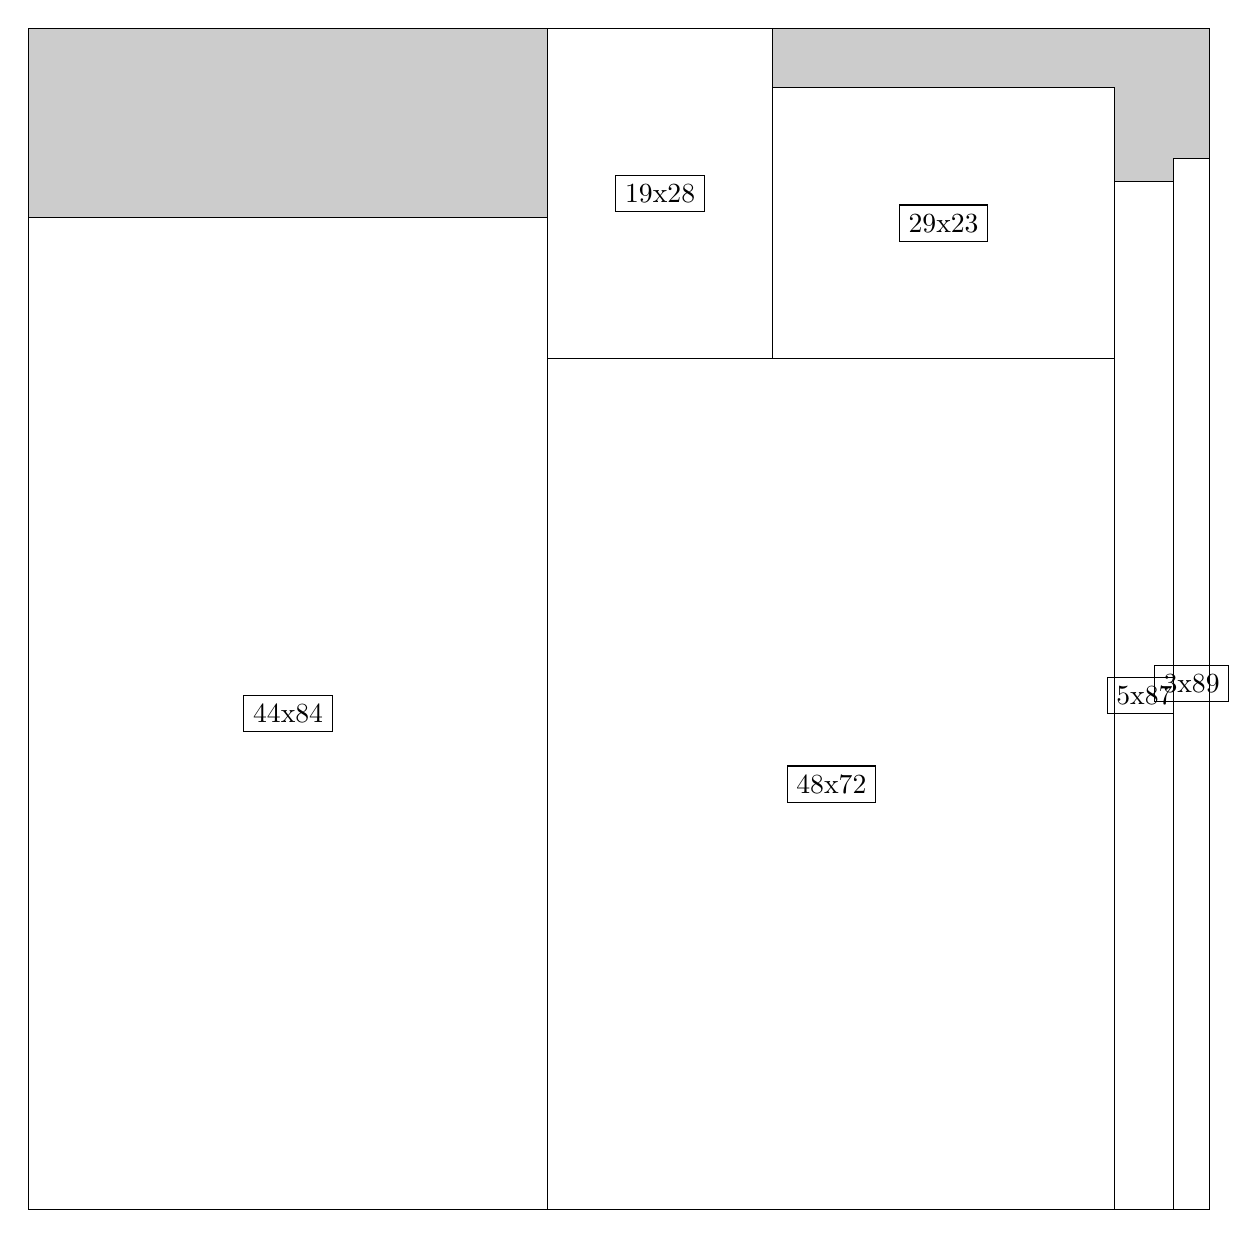
\begin{tikzpicture}[shorten >=1pt,scale=1.0,every node/.style={scale=1.0},->]
\tikzstyle{vertex}=[circle,fill=black!25,minimum size=14pt,inner sep=0pt]
\filldraw[fill=gray!40!white, draw=black] (0,0) rectangle (15.0,15.0);
\foreach \name/\x/\y/\w/\h in {44x84/0.0/0.0/6.6/12.6,48x72/6.6/0.0/7.199999999999999/10.799999999999999,29x23/9.45/10.799999999999999/4.35/3.4499999999999997,19x28/6.6/10.799999999999999/2.85/4.2,5x87/13.799999999999999/0.0/0.75/13.049999999999999,3x89/14.549999999999999/0.0/0.44999999999999996/13.35}
\filldraw[fill=white!40!white, draw=black] (\x,\y) rectangle node[draw] (\name) {\name} ++(\w,\h);
\end{tikzpicture}


w =44 , h =84 , x =0 , y =0 , v =3696
\par
w =48 , h =72 , x =44 , y =0 , v =3456
\par
w =29 , h =23 , x =63 , y =72 , v =667
\par
w =19 , h =28 , x =44 , y =72 , v =532
\par
w =5 , h =87 , x =92 , y =0 , v =435
\par
w =3 , h =89 , x =97 , y =0 , v =267
\par
\newpage


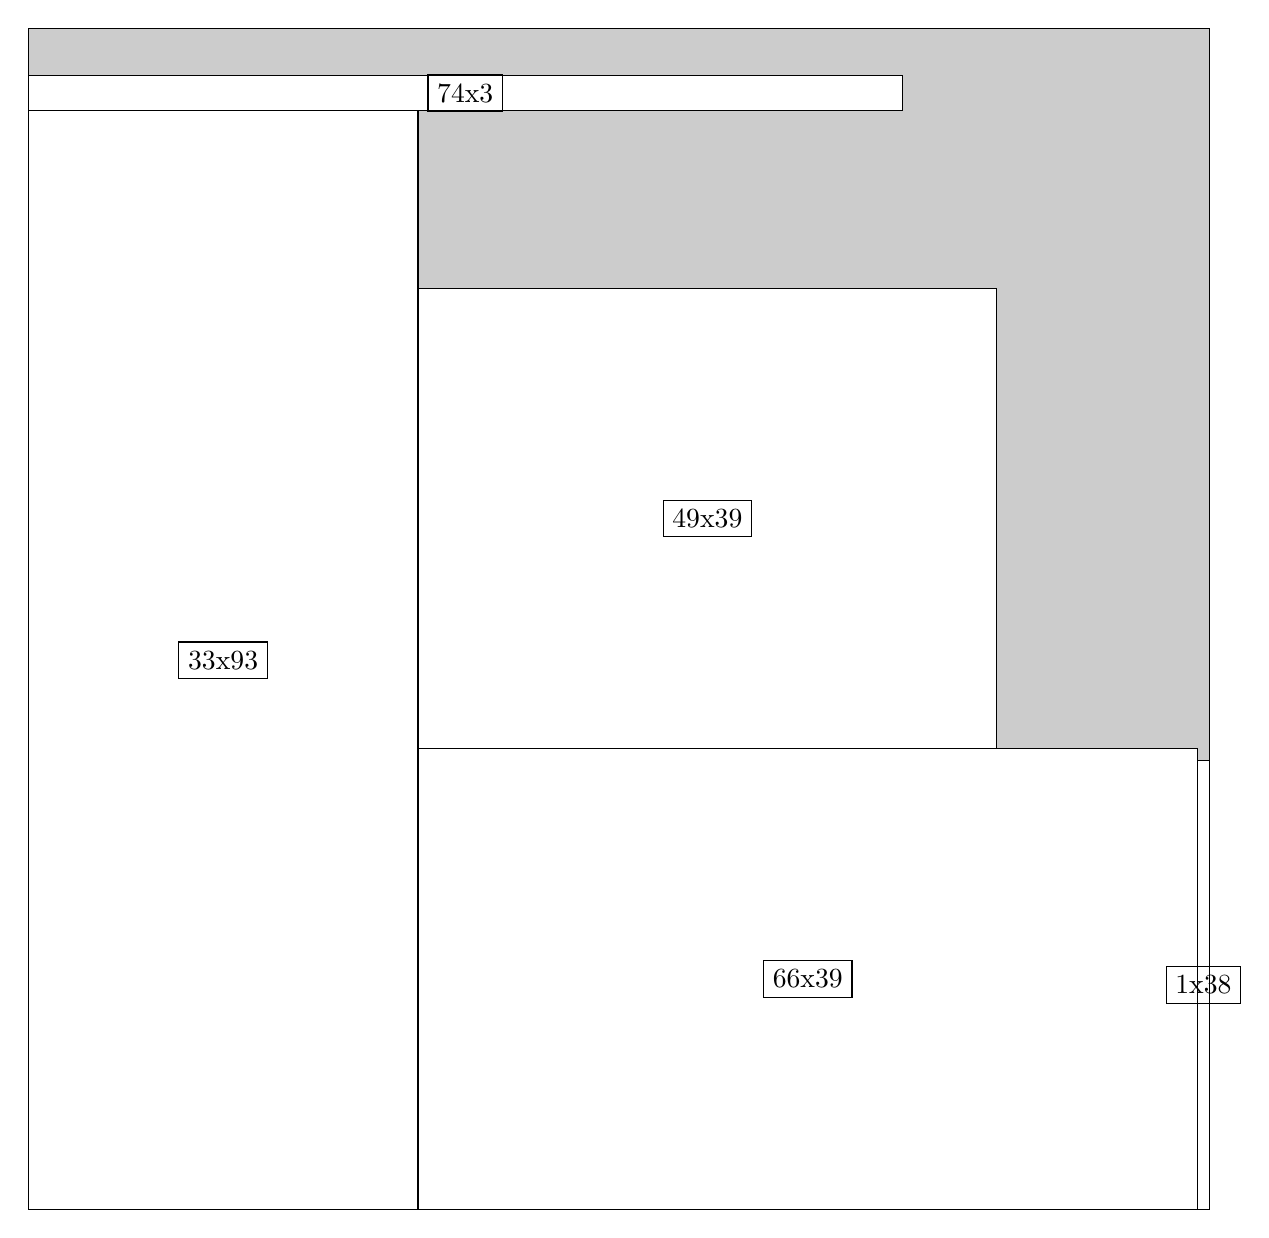
\begin{tikzpicture}[shorten >=1pt,scale=1.0,every node/.style={scale=1.0},->]
\tikzstyle{vertex}=[circle,fill=black!25,minimum size=14pt,inner sep=0pt]
\filldraw[fill=gray!40!white, draw=black] (0,0) rectangle (15.0,15.0);
\foreach \name/\x/\y/\w/\h in {33x93/0.0/0.0/4.95/13.95,66x39/4.95/0.0/9.9/5.85,49x39/4.95/5.85/7.35/5.85,74x3/0.0/13.95/11.1/0.44999999999999996,1x38/14.85/0.0/0.15/5.7}
\filldraw[fill=white!40!white, draw=black] (\x,\y) rectangle node[draw] (\name) {\name} ++(\w,\h);
\end{tikzpicture}


w =33 , h =93 , x =0 , y =0 , v =3069
\par
w =66 , h =39 , x =33 , y =0 , v =2574
\par
w =49 , h =39 , x =33 , y =39 , v =1911
\par
w =74 , h =3 , x =0 , y =93 , v =222
\par
w =1 , h =38 , x =99 , y =0 , v =38
\par
\newpage


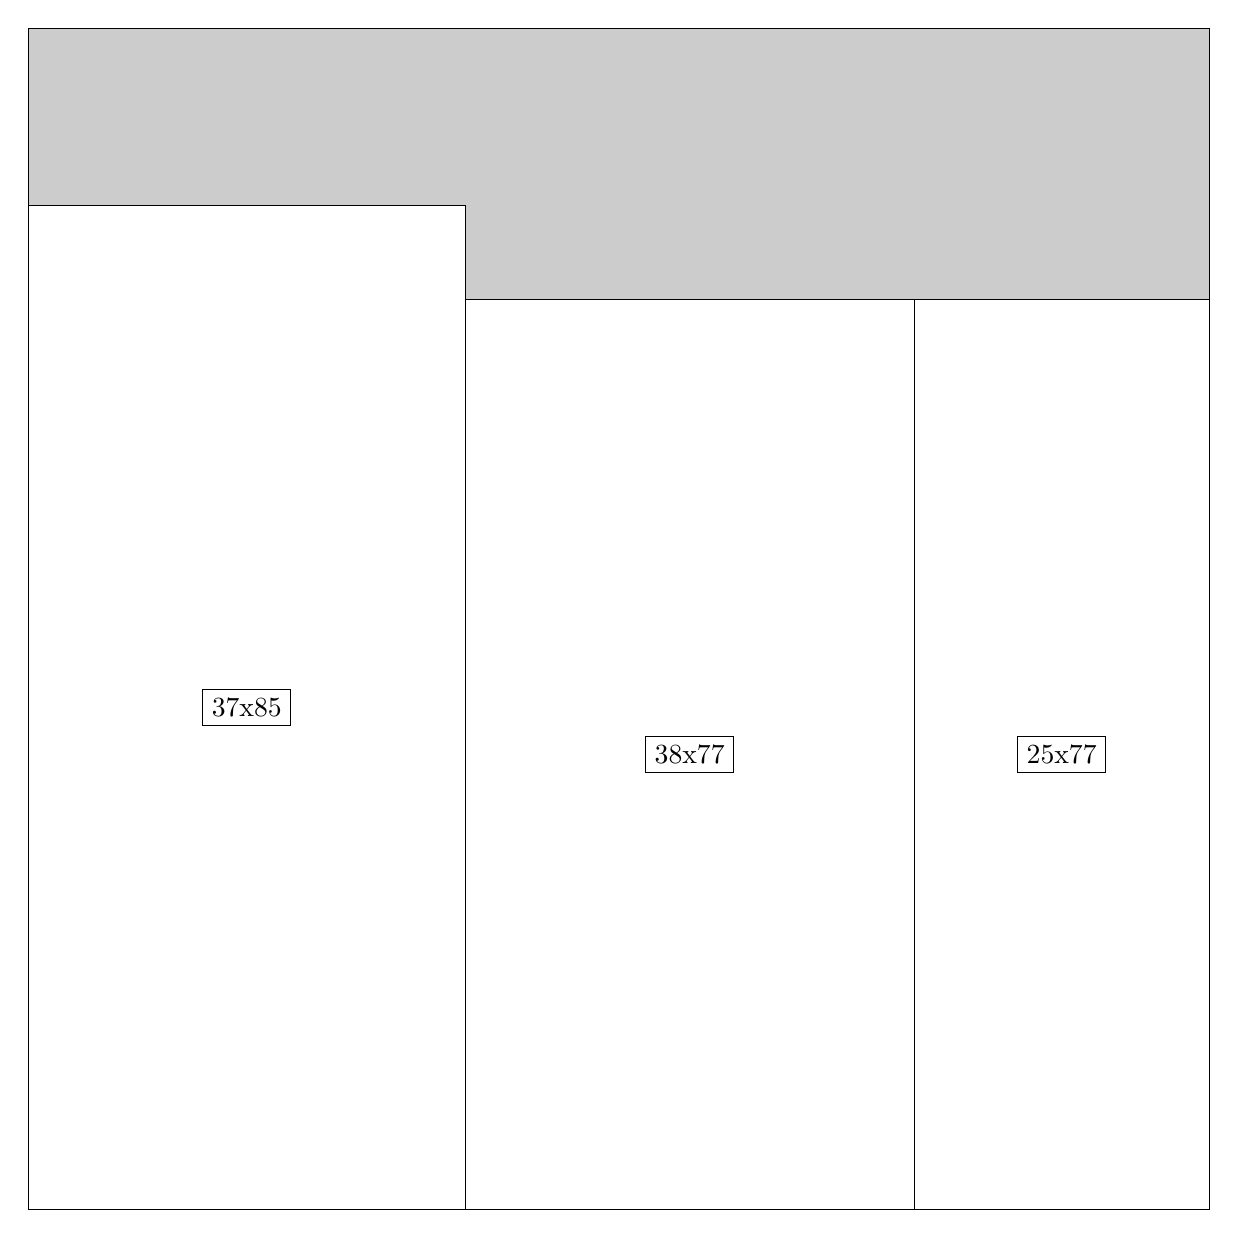
\begin{tikzpicture}[shorten >=1pt,scale=1.0,every node/.style={scale=1.0},->]
\tikzstyle{vertex}=[circle,fill=black!25,minimum size=14pt,inner sep=0pt]
\filldraw[fill=gray!40!white, draw=black] (0,0) rectangle (15.0,15.0);
\foreach \name/\x/\y/\w/\h in {37x85/0.0/0.0/5.55/12.75,38x77/5.55/0.0/5.7/11.549999999999999,25x77/11.25/0.0/3.75/11.549999999999999}
\filldraw[fill=white!40!white, draw=black] (\x,\y) rectangle node[draw] (\name) {\name} ++(\w,\h);
\end{tikzpicture}


w =37 , h =85 , x =0 , y =0 , v =3145
\par
w =38 , h =77 , x =37 , y =0 , v =2926
\par
w =25 , h =77 , x =75 , y =0 , v =1925
\par
\newpage


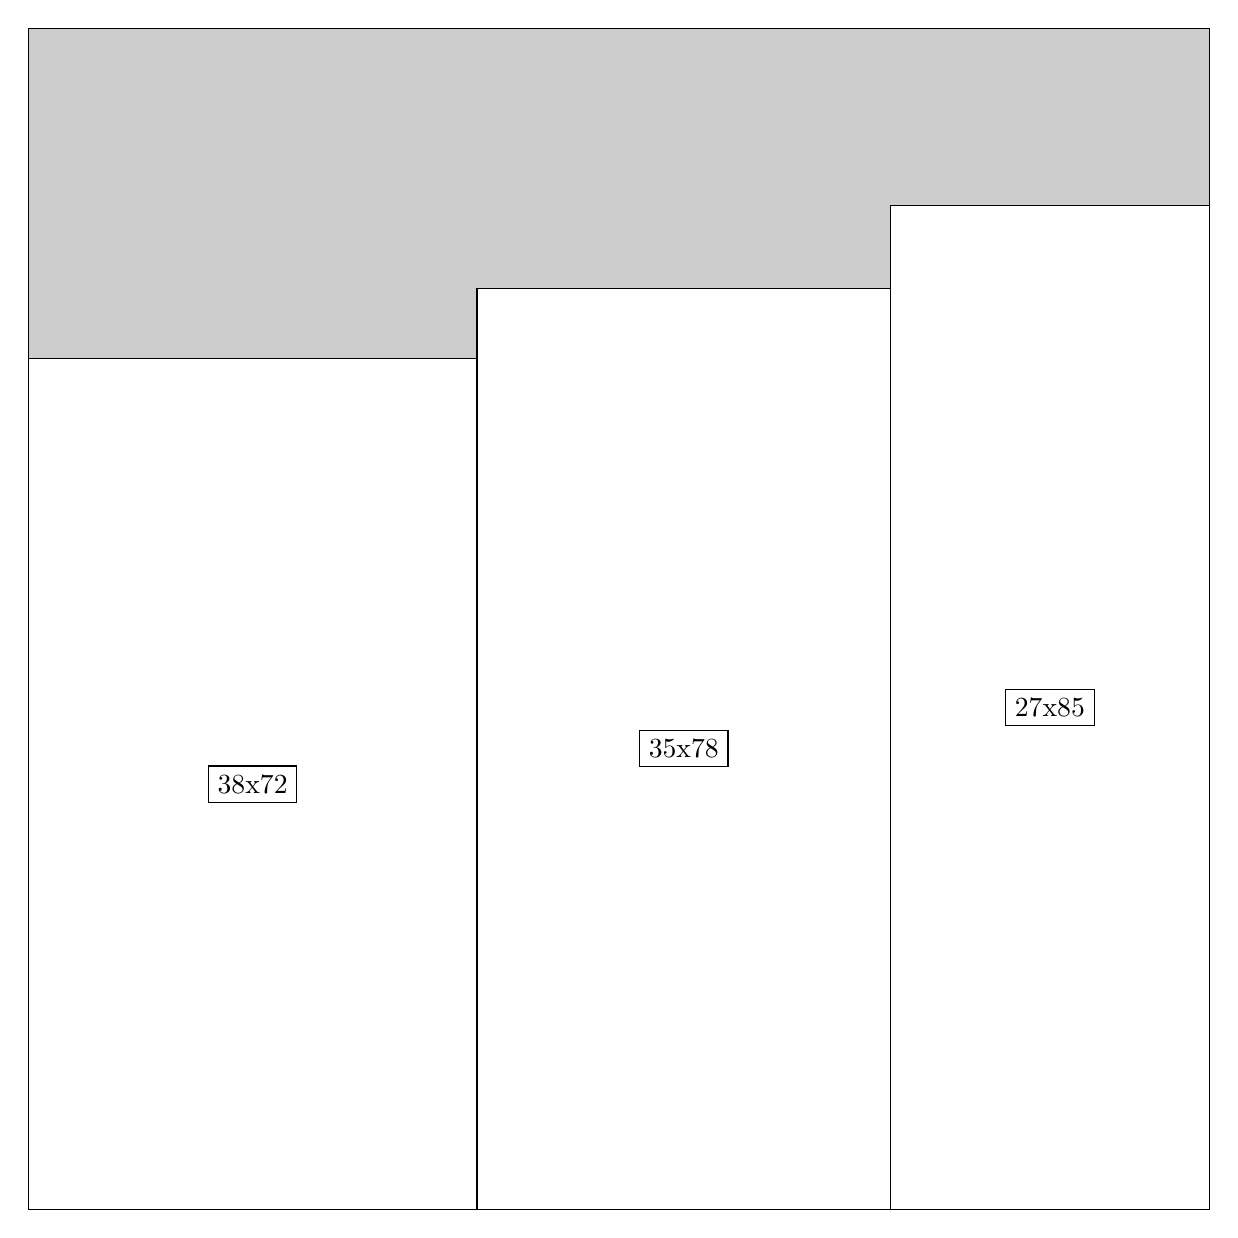
\begin{tikzpicture}[shorten >=1pt,scale=1.0,every node/.style={scale=1.0},->]
\tikzstyle{vertex}=[circle,fill=black!25,minimum size=14pt,inner sep=0pt]
\filldraw[fill=gray!40!white, draw=black] (0,0) rectangle (15.0,15.0);
\foreach \name/\x/\y/\w/\h in {38x72/0.0/0.0/5.7/10.799999999999999,35x78/5.7/0.0/5.25/11.7,27x85/10.95/0.0/4.05/12.75}
\filldraw[fill=white!40!white, draw=black] (\x,\y) rectangle node[draw] (\name) {\name} ++(\w,\h);
\end{tikzpicture}


w =38 , h =72 , x =0 , y =0 , v =2736
\par
w =35 , h =78 , x =38 , y =0 , v =2730
\par
w =27 , h =85 , x =73 , y =0 , v =2295
\par
\newpage


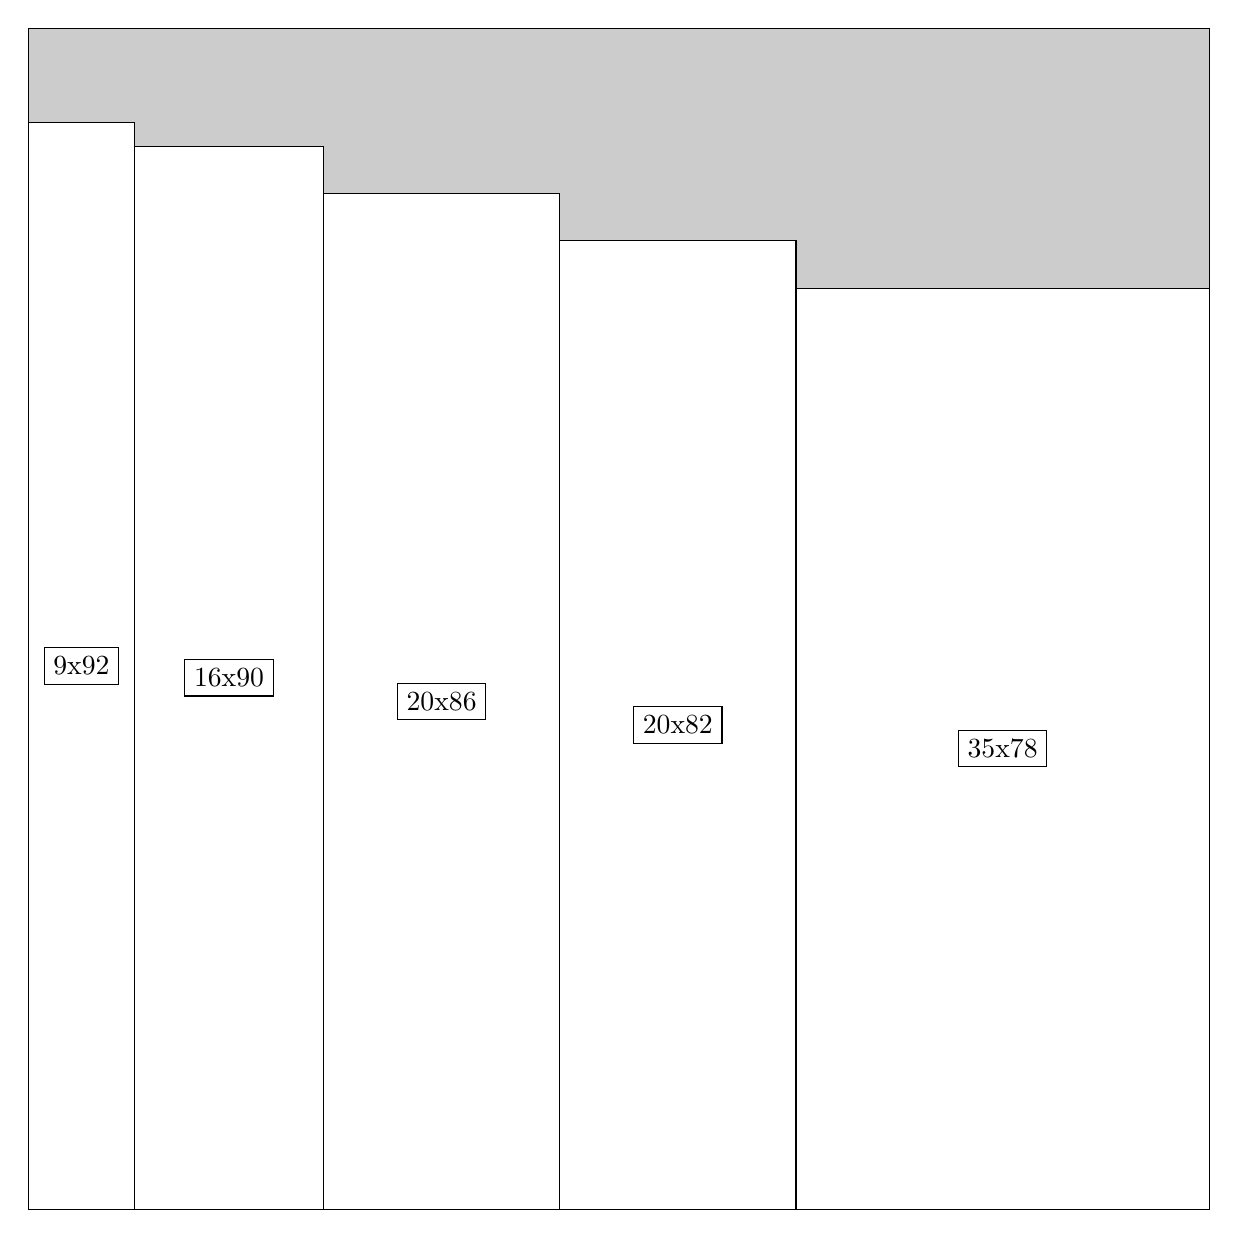
\begin{tikzpicture}[shorten >=1pt,scale=1.0,every node/.style={scale=1.0},->]
\tikzstyle{vertex}=[circle,fill=black!25,minimum size=14pt,inner sep=0pt]
\filldraw[fill=gray!40!white, draw=black] (0,0) rectangle (15.0,15.0);
\foreach \name/\x/\y/\w/\h in {20x86/3.75/0.0/3.0/12.9,20x82/6.75/0.0/3.0/12.299999999999999,35x78/9.75/0.0/5.25/11.7,16x90/1.3499999999999999/0.0/2.4/13.5,9x92/0.0/0.0/1.3499999999999999/13.799999999999999}
\filldraw[fill=white!40!white, draw=black] (\x,\y) rectangle node[draw] (\name) {\name} ++(\w,\h);
\end{tikzpicture}


w =20 , h =86 , x =25 , y =0 , v =1720
\par
w =20 , h =82 , x =45 , y =0 , v =1640
\par
w =35 , h =78 , x =65 , y =0 , v =2730
\par
w =16 , h =90 , x =9 , y =0 , v =1440
\par
w =9 , h =92 , x =0 , y =0 , v =828
\par
\newpage


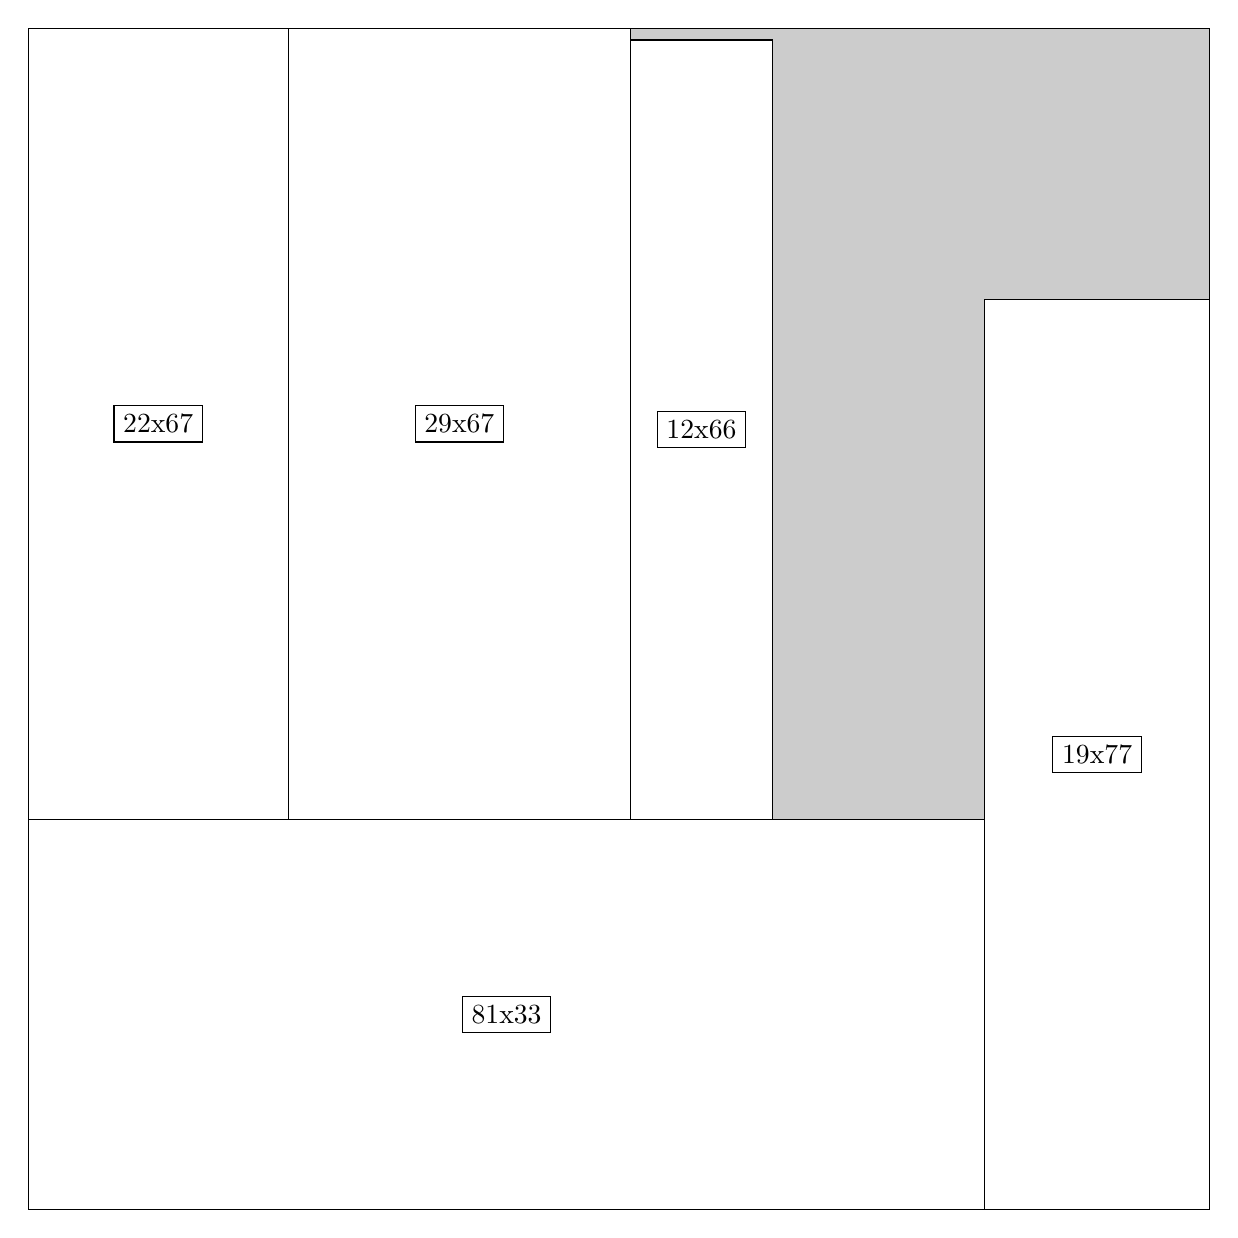
\begin{tikzpicture}[shorten >=1pt,scale=1.0,every node/.style={scale=1.0},->]
\tikzstyle{vertex}=[circle,fill=black!25,minimum size=14pt,inner sep=0pt]
\filldraw[fill=gray!40!white, draw=black] (0,0) rectangle (15.0,15.0);
\foreach \name/\x/\y/\w/\h in {81x33/0.0/0.0/12.15/4.95,29x67/3.3/4.95/4.35/10.049999999999999,22x67/0.0/4.95/3.3/10.049999999999999,19x77/12.15/0.0/2.85/11.549999999999999,12x66/7.6499999999999995/4.95/1.7999999999999998/9.9}
\filldraw[fill=white!40!white, draw=black] (\x,\y) rectangle node[draw] (\name) {\name} ++(\w,\h);
\end{tikzpicture}


w =81 , h =33 , x =0 , y =0 , v =2673
\par
w =29 , h =67 , x =22 , y =33 , v =1943
\par
w =22 , h =67 , x =0 , y =33 , v =1474
\par
w =19 , h =77 , x =81 , y =0 , v =1463
\par
w =12 , h =66 , x =51 , y =33 , v =792
\par
\newpage


\end{document}